	% .:: Laden der LaTeX4EI Formelsammlungsvorlage
\documentclass[fs, footer]{latex4ei}

% Dokumentbeginn
% ======================================================================
\begin{document}


% Aufteilung in Spalten
\begin{multicols*}{4}



% -------------------------------------------
% | 		Leistungselektronik			    |
% ~~~~~~~~~~~~~~~~~~~~~~~~~~~~~~~~~~~~~~~~~~~
\fstitle{Leistungselektronik}

\section*{Allgemeines}

\sectionbox{
Mittelwert: $u_{\ir M} =  \frac{1}{T} \int \limits_{t_0}^{t_0 + T} u(t) \diff t$

Effektivwert (RMS): $	U_{\ir eff} = \frac 1 T \sqrt{ \int \limits_{0}^{T} u^2(t) \diff t}$
}





\section{Grundlagen}

\sectionbox{
\subsection{Elektrische Engergieumwandlung durch Stromrichter}
\begin{center}
	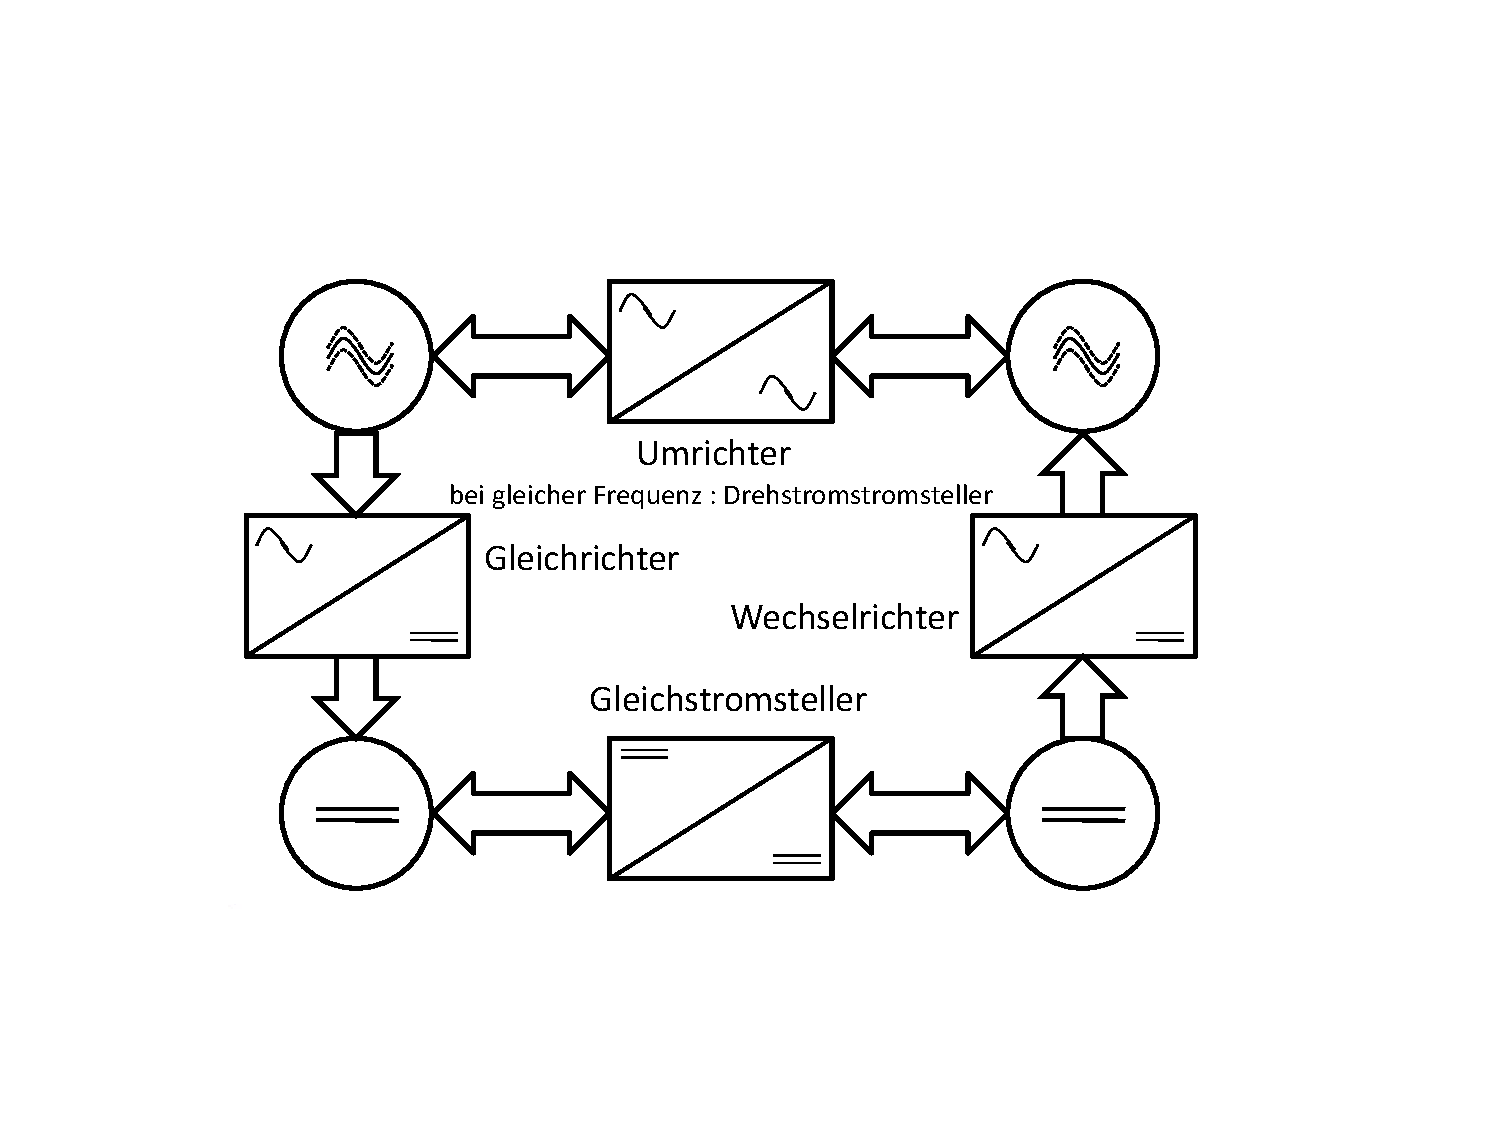
\includegraphics[width=6cm]{img/1-Energiewandlung.pdf}
\end{center}

}

\section{Leistungshalbleiter}
\sectionbox{b
aktiver Betrieb von Halbleitern wird bewusst vermieden.

Leistungshalbleiter sind keine idealen Schalter $\ra$ Verluste

\subsection{Hartschaltende Bauelemente}
\begin{itemize}
	\item Sehr hohe Halbleiterbelastung
	\item Große Safe Operating Area erforderlich
	\item Niedrige Schaltfrequenz
	\item Problematisch bei hohen Leistungen
\end{itemize}

\subsection{Weichschaltende Bauelemente}
\begin{itemize}
	\item Niedrige Halbleiterbelastung
	\item Höherer Ausschaltstrom
	\item Hohe Schaltfrequenz
	\item Einfacherer Gate-Treiber
	\item Zusätzliche Leistungskomponenten
\end{itemize}
}

\section{Kühlung von Leistungshalbleitern}
\sectionbox{
	Abgestrahlte Leistung: $P_{\ir rad} = \sigma \epsilon A (T^4_{KK} - T^4_{a})$
	
	Strahlungskonstante: $\sigma = 5,67 \cdot 10^{-8} \si{\watt \per \meter \squared \kelvin \tothe 4}$
	
}

\section{Netzgefuehrte Schaltungen}
\sectionbox{

\subsection{Netzteile}

Grundstruktur

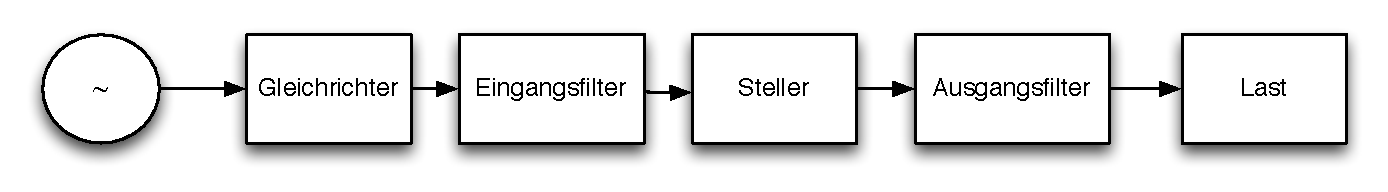
\includegraphics[width=7cm]{img/03-Grundstruktur.pdf}

\paragraph{Gleichrichter} 
Gleichrichterschaltungen unterscheidet man in Mittelpunkt- und Brückenschaltungen. Außerdem unterscheidet man aufgrund der Anzahl an Kommutierungen pro Periode.



\paragraph{Hinweis:}
An einer (idealen)Diode können nur positive Ströme auftreten. Allerdings ist (bei induktiven Lasten) das auftreten von negativen Spannungen möglich.

$\Ra$ die Ausgangsspannung hängt immer auch von der Art der Last ab!

mit Freilaufdiode

\begin{center}
	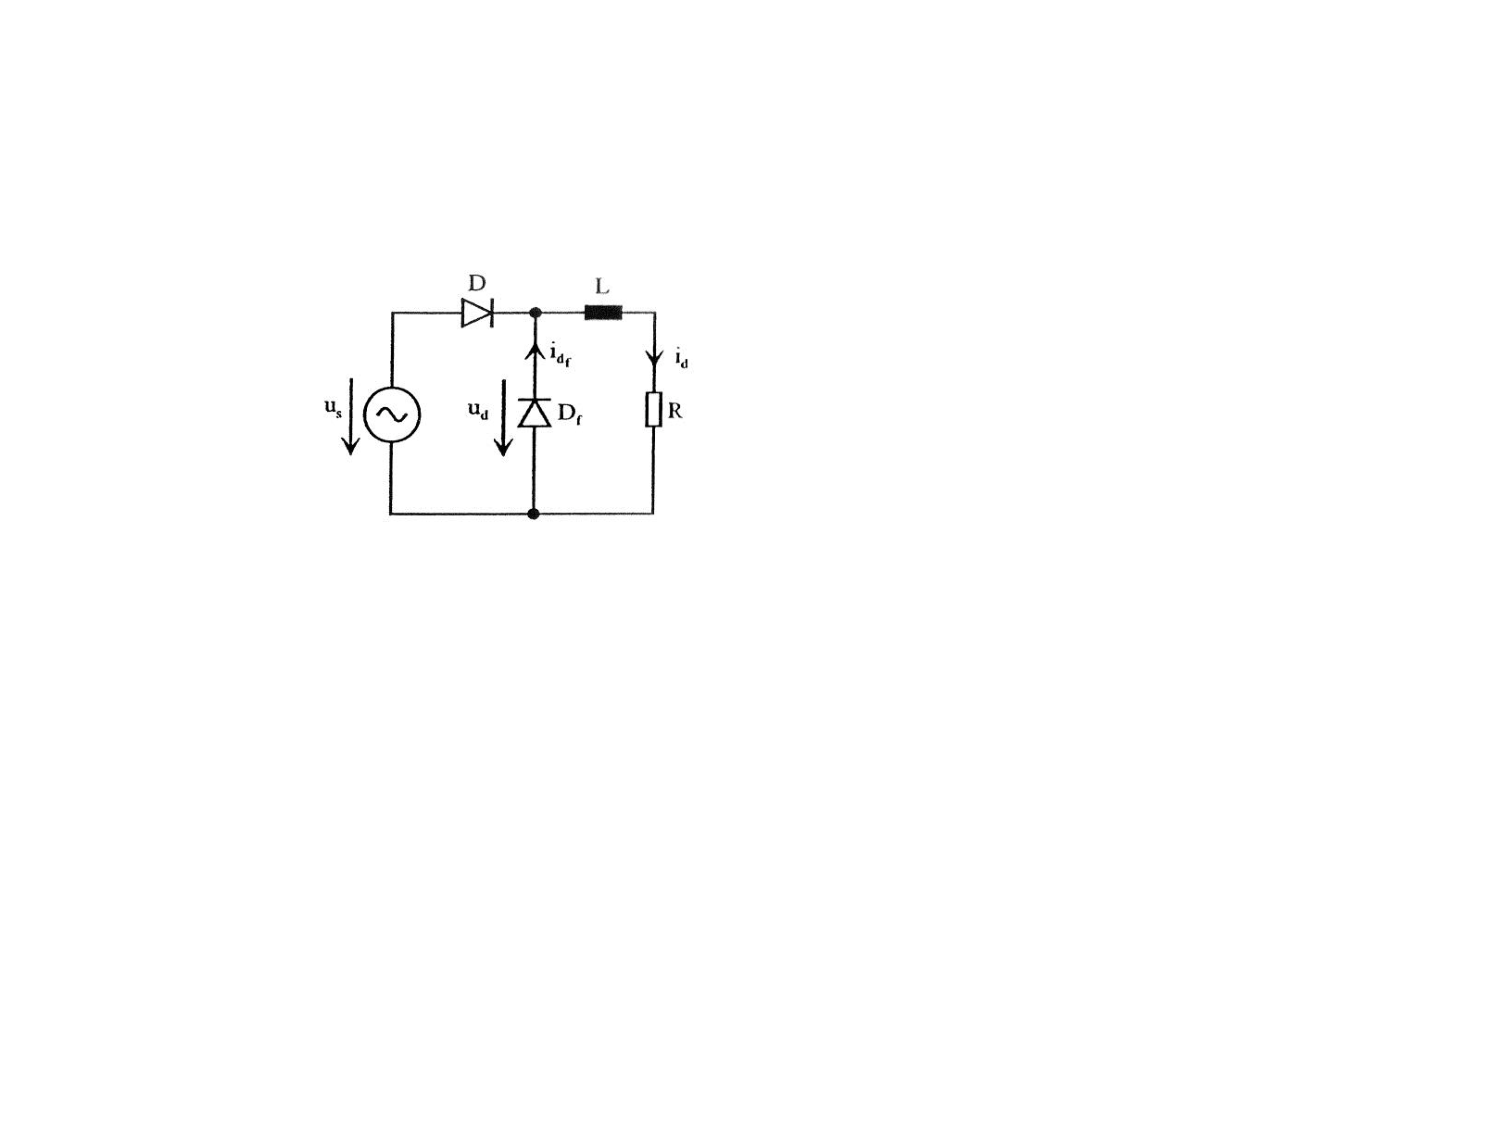
\includegraphics[width=5cm]{img/03-mit_Freilauf.pdf}
\end{center}
}

\sectionbox{

\subsection{B2-Schaltung (Graetz-Brücke)}
mit Transformator zur galvanischen Trennung. \\ 

für $U > 0$: $i$ fließt über $D1$, Last, $D4$

für $U < 0$: $i$ fließt über $D2$, Last, $D3$

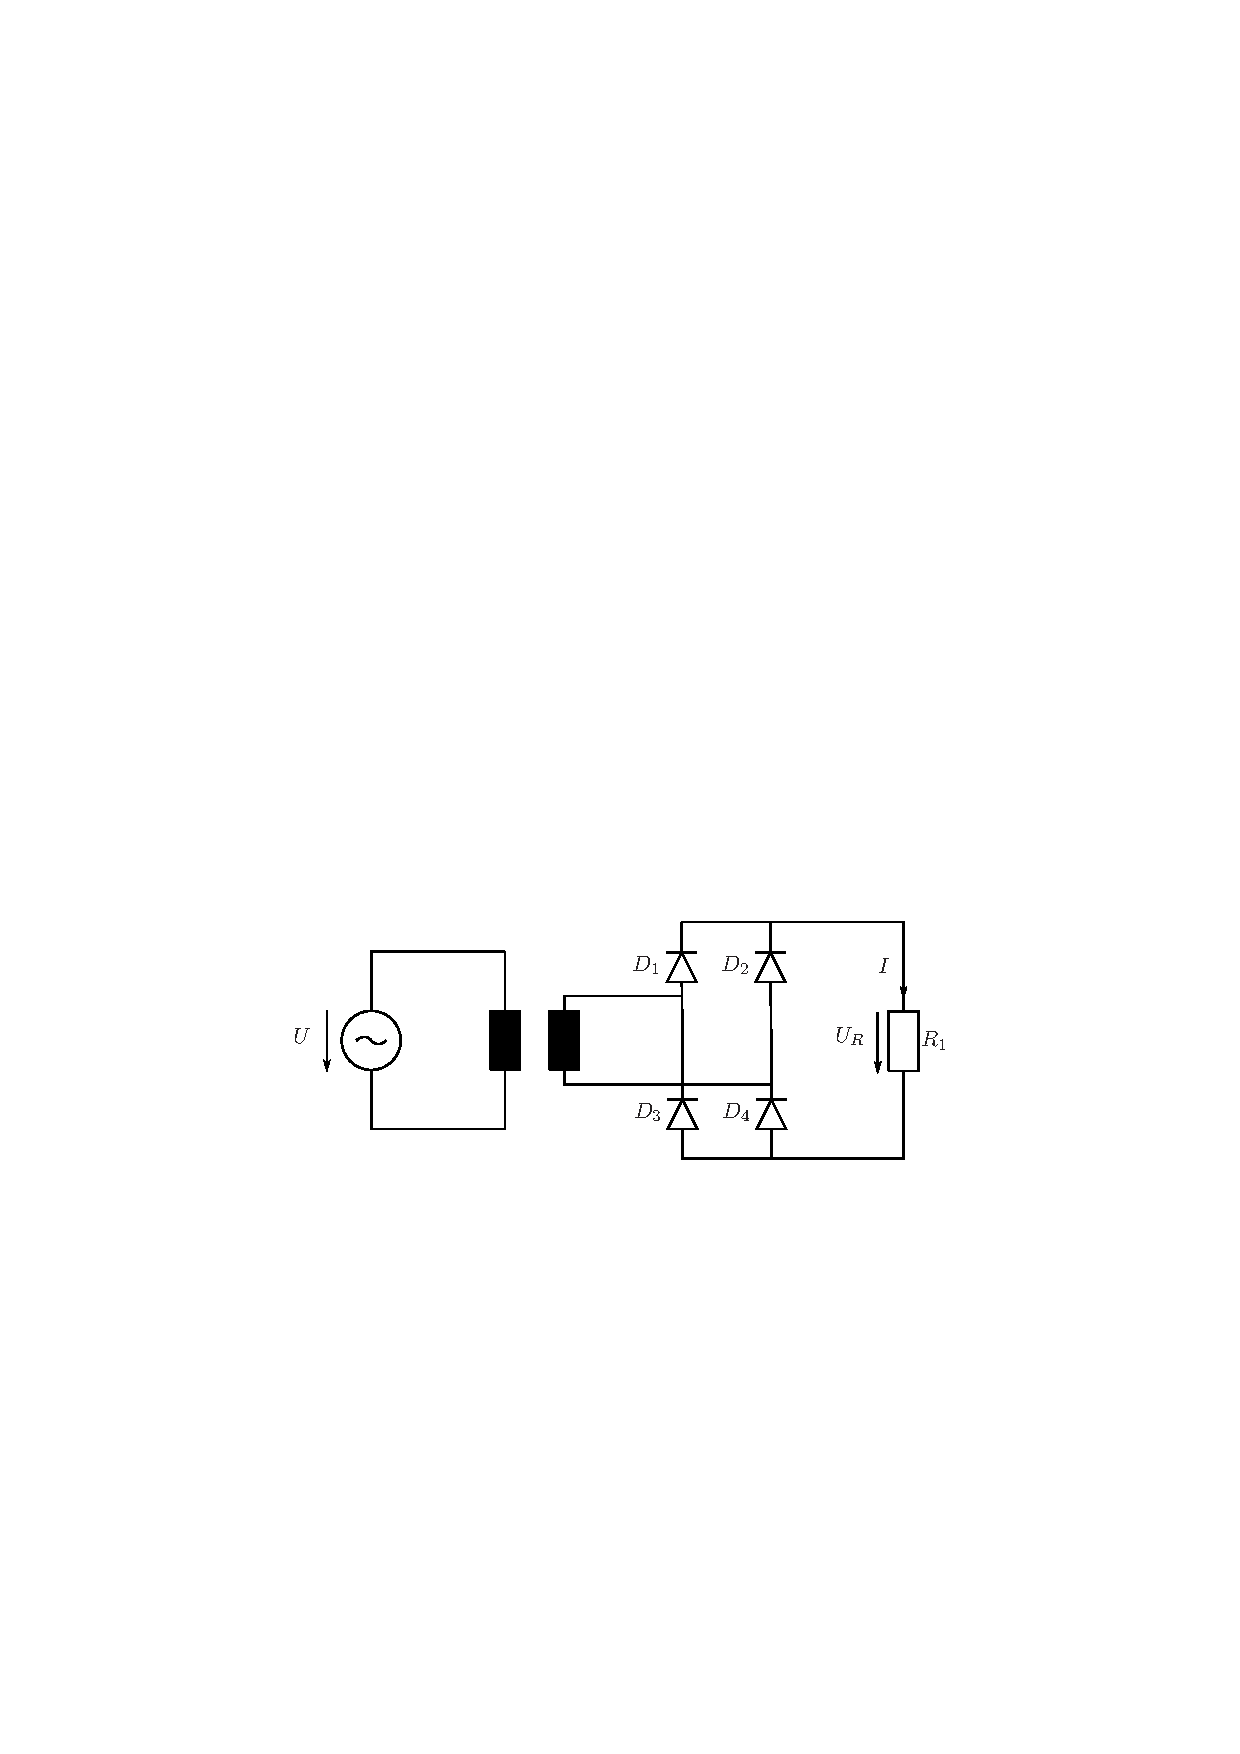
\includegraphics[width=7cm]{img/B2-Schaltung.pdf}

\tablebox{
\begin{tabular}{lll}
\ctrule
Last & Strom & Spannung \\ \cmrule
R & - & - \\
RL &Glättung: wird nicht zu null& gleichgerichteter Sinus \\
RC & hoher Aufladestrom & Glättung: sinkt langsam ab \\
\cbrule
\end{tabular}
} \\ 

Voltage Ripple: $U_{\ir max} - U_{\ir min}$ \\

\symbolbox{
\begin{tabular}{ll}
$a$ & Zahl der ausfallenden Halbswellen \\
$f$ & Frequenz der Halbwelle
\end{tabular}
}
\cookbox{Dimensionierung des Glättungskondensators}{
	\item Festlegung $I_{\ir max}$
	\item Festlegung Voltage Ripple oder min. Spannung
	
		$\Ra $ Ladepausendauer = 1 Halbwelle
	\item Ausfallende Halbwellen?
	
		$\Ra$ $t_{\ir LP} \approx (a + 1) \frac 1 f$
	\item Kondensator: $i = C \frac{\diff u}{\diff t} $ \quad $i = I_{\ir max} = const.$
	
	$C = \frac{I_{\ir max} t_{\ir LP}}{\hat{U} - U_{\ir min}}$
}
}

\sectionbox{
\subsection{M3-Schaltung}
Es leitet immer die Diode mit dem höchsten Potential.

\begin{center}
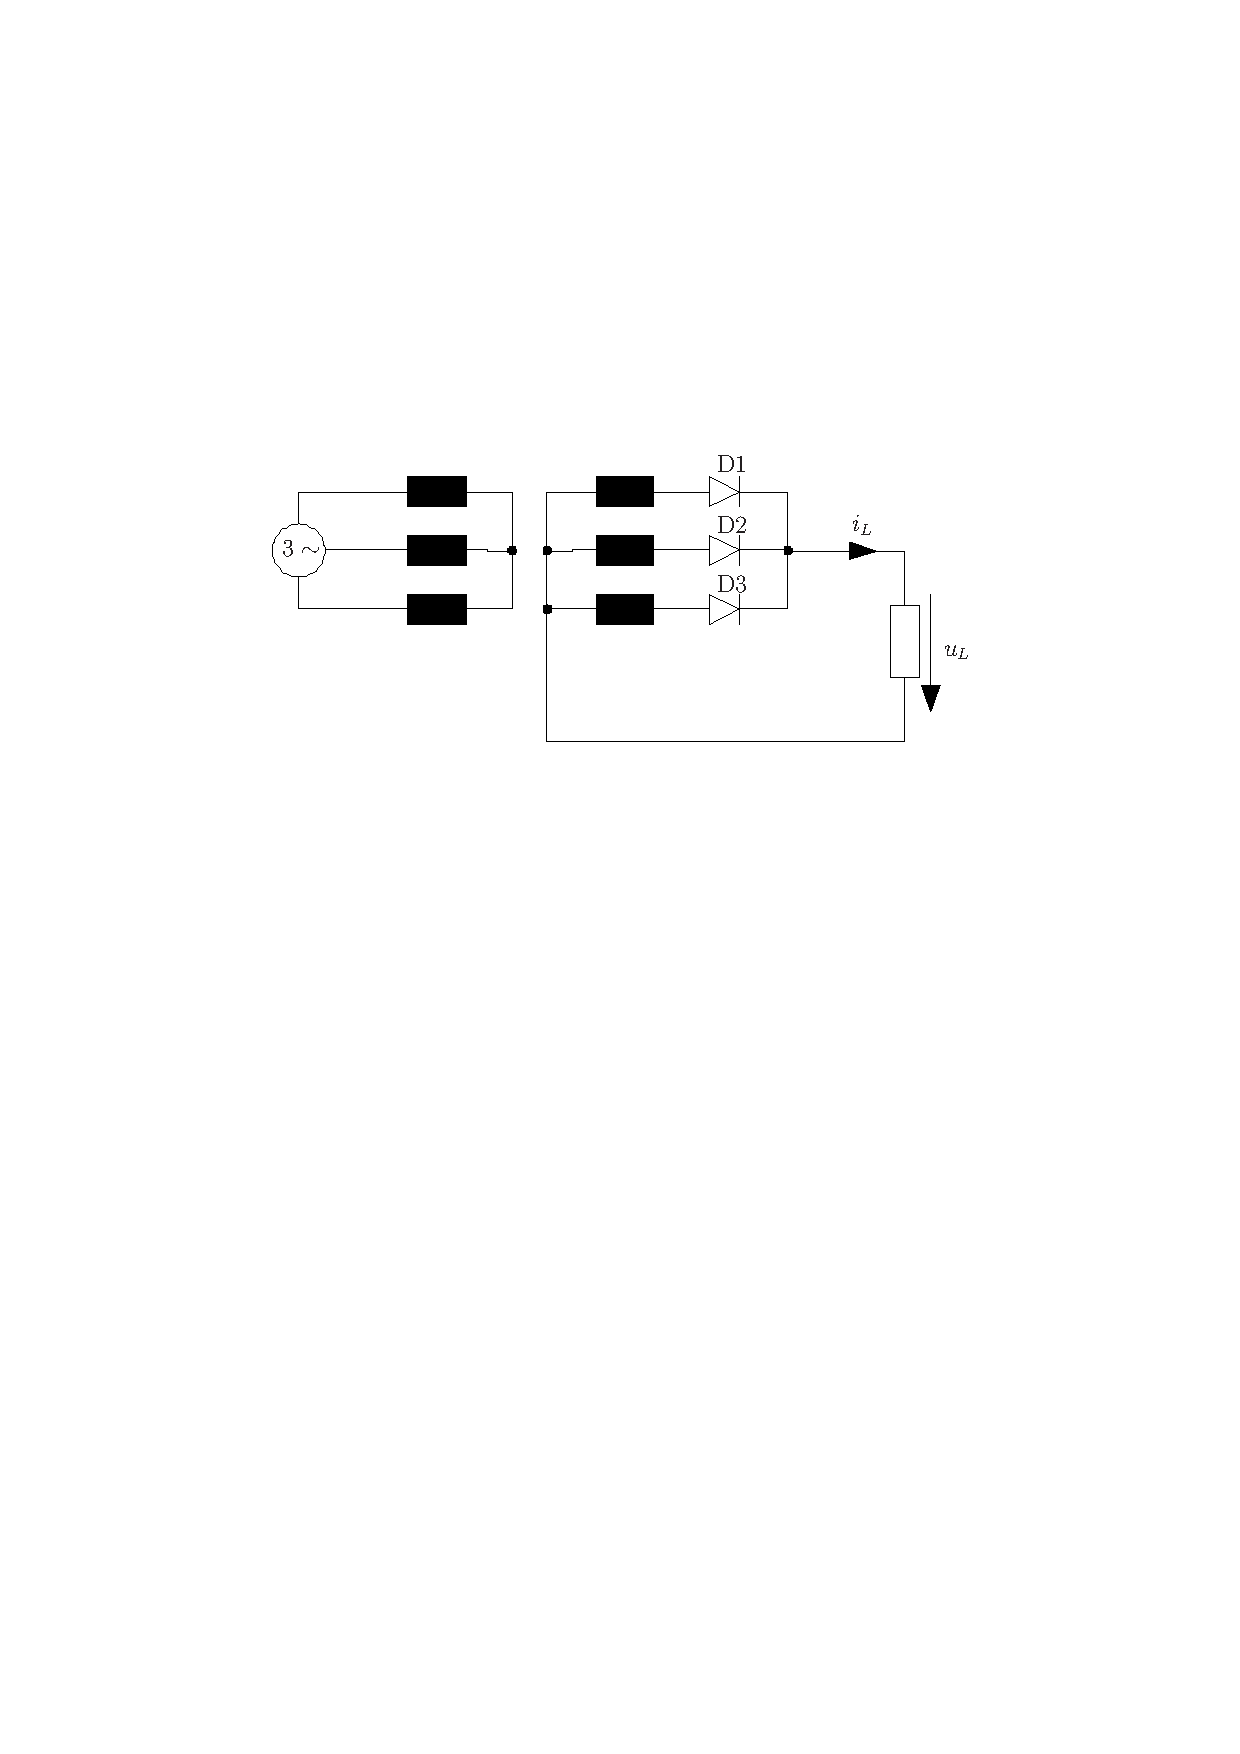
\includegraphics[width=5cm]{img/03-M3-Schaltung.pdf}

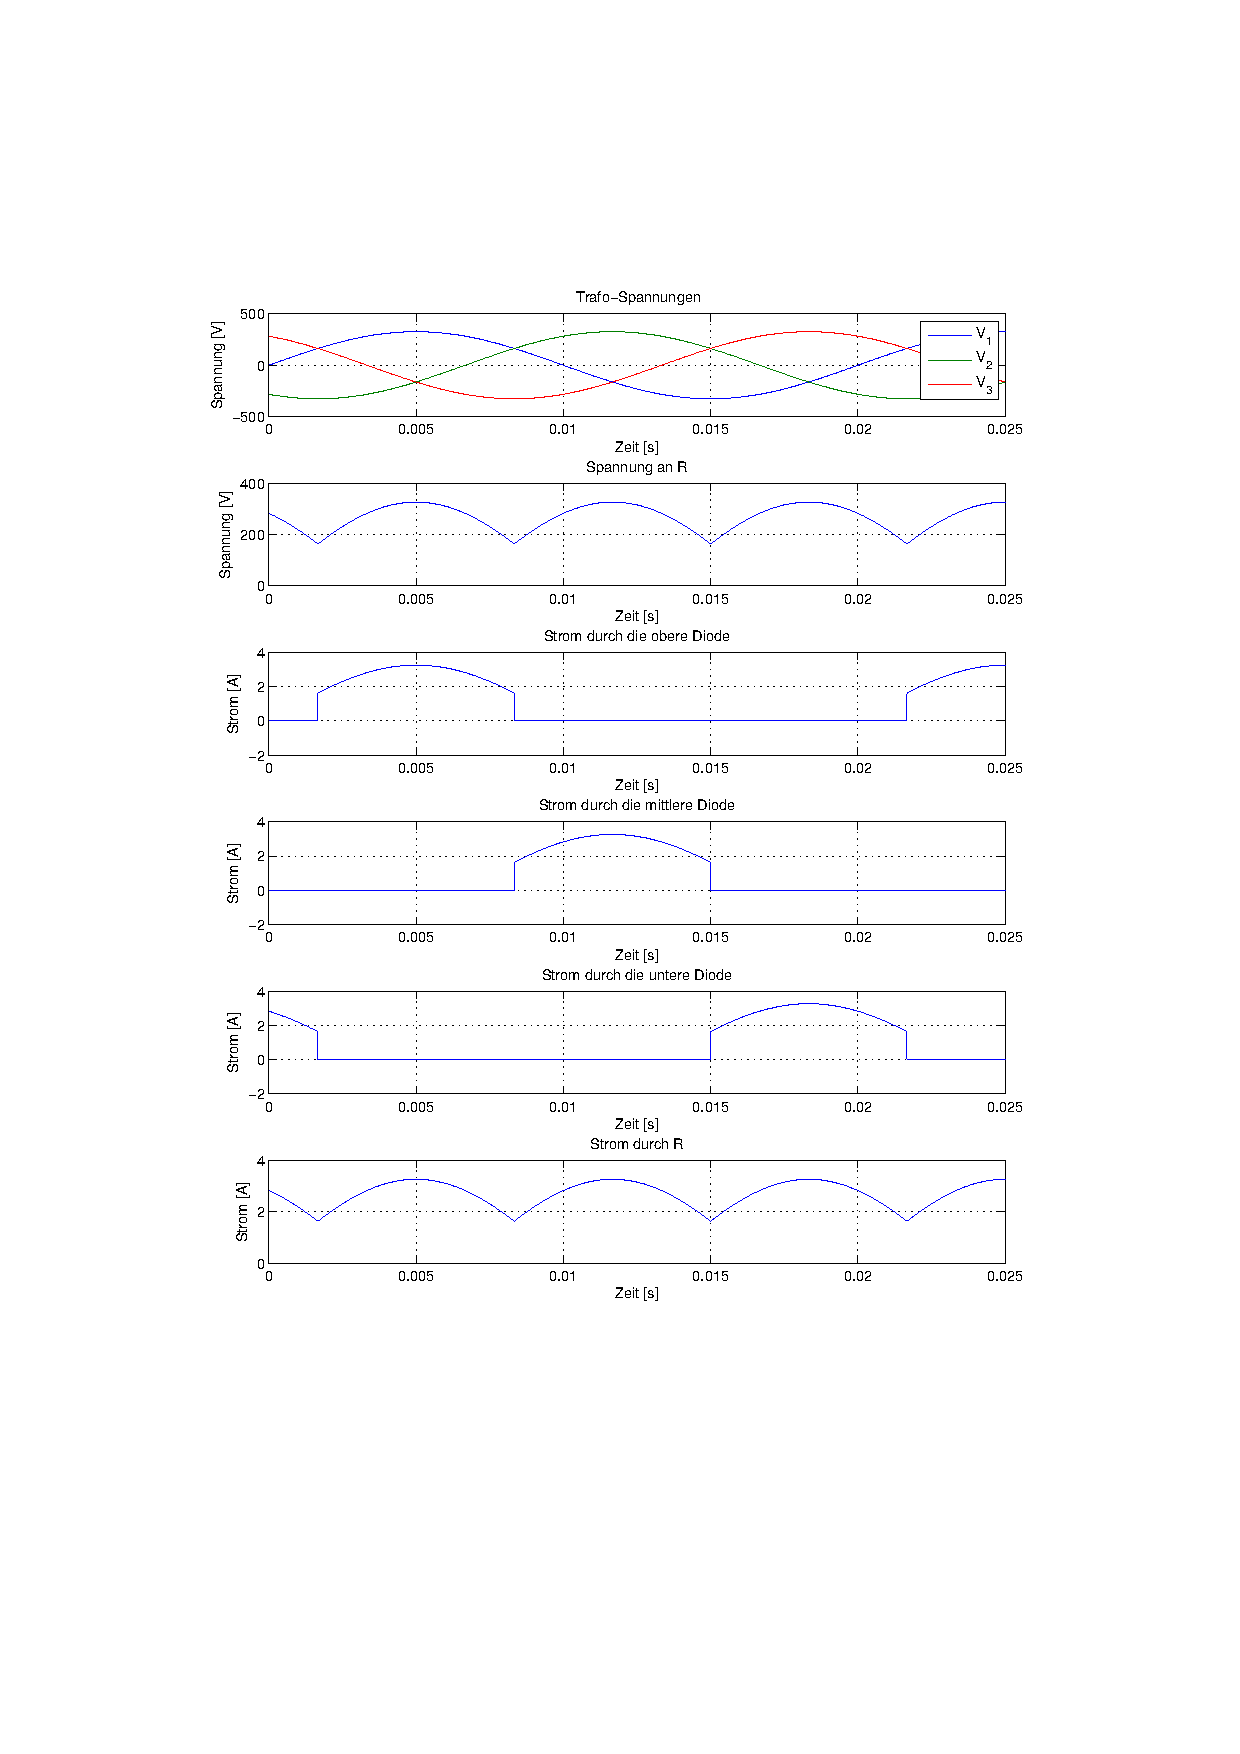
\includegraphics[width=6cm]{img/03-M3-Spannungsverlauf.pdf}

\end{center}
}

\sectionbox{
\subsection{B6-Schaltung}

Oben: Es leitet immer die Diode mit dem höchsten Potential.

Unten: Es leitet immer die Diode mit dem niedrigsten Potential.

	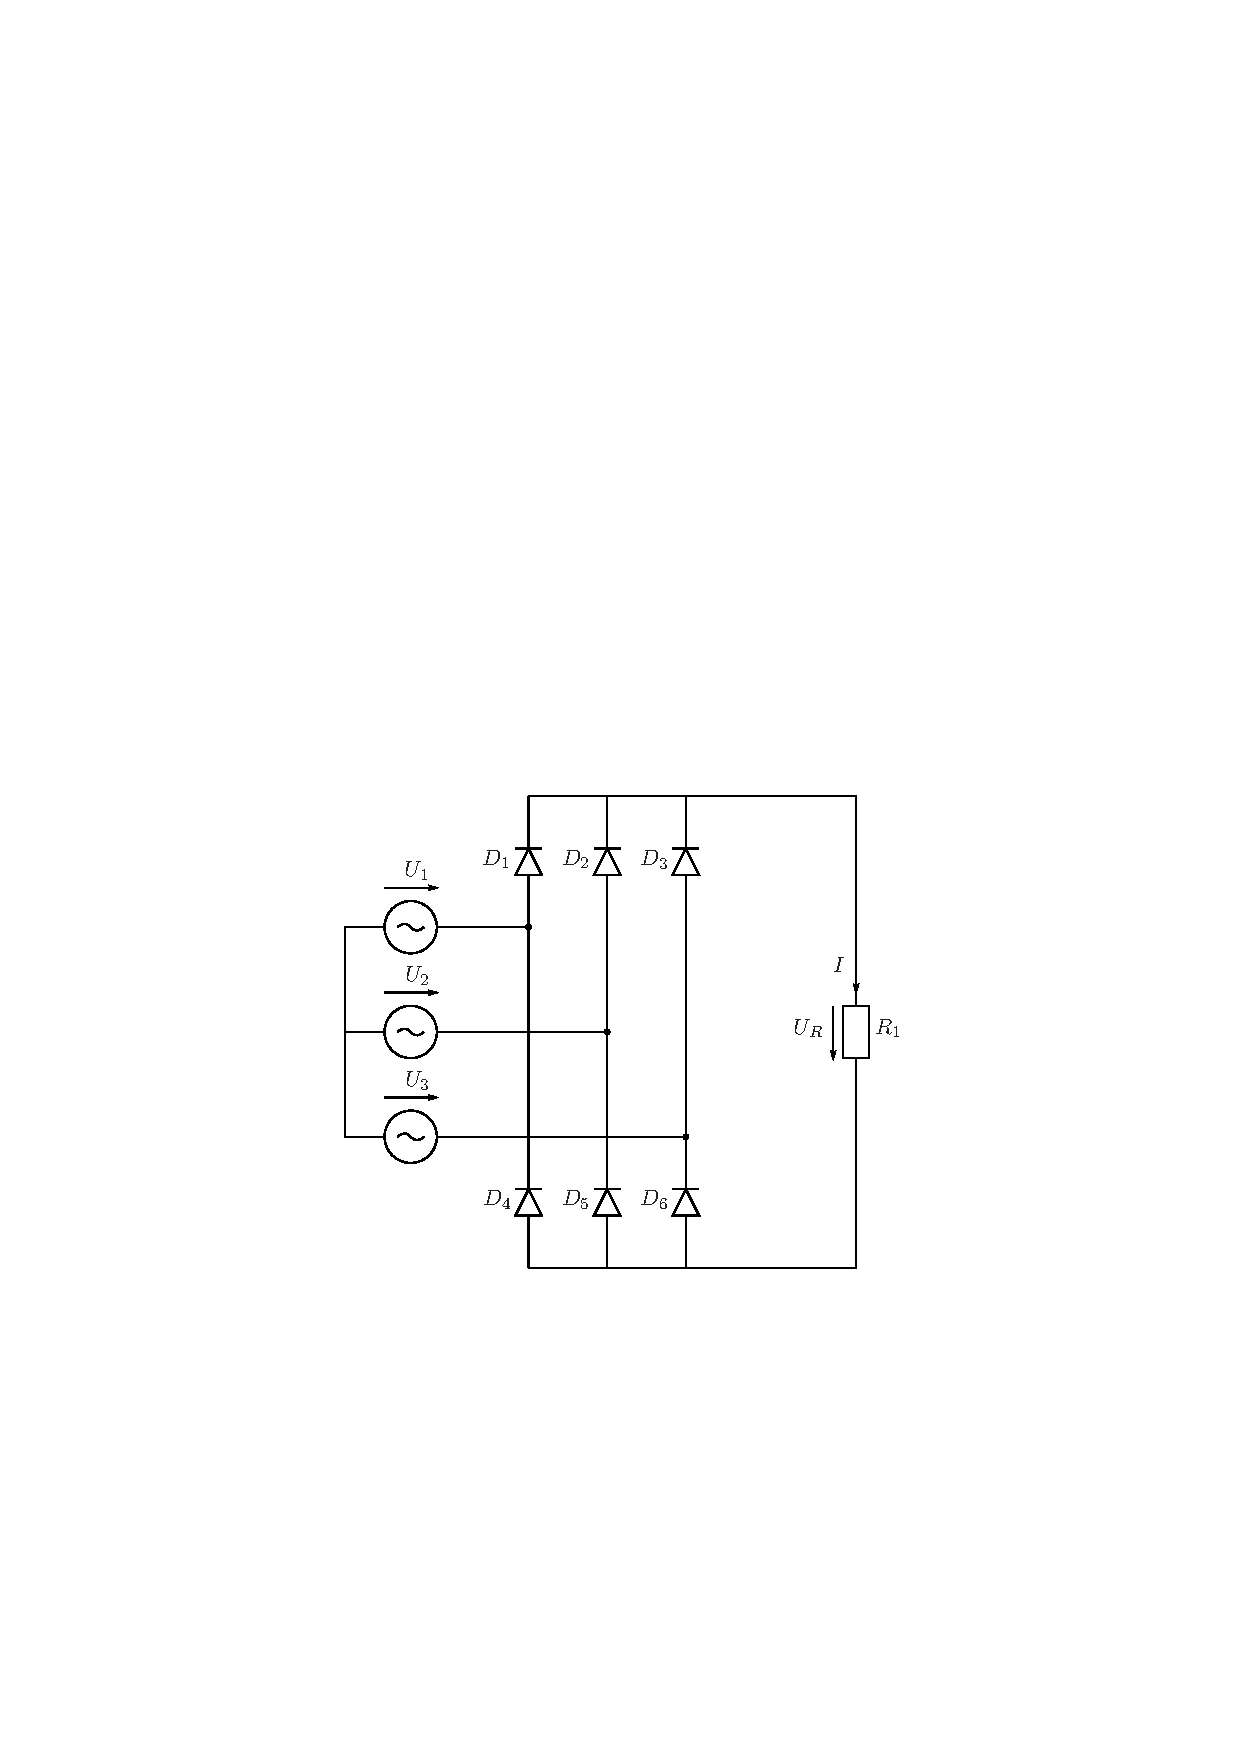
\includegraphics[width=5cm]{img/B6-Schaltung.pdf}
	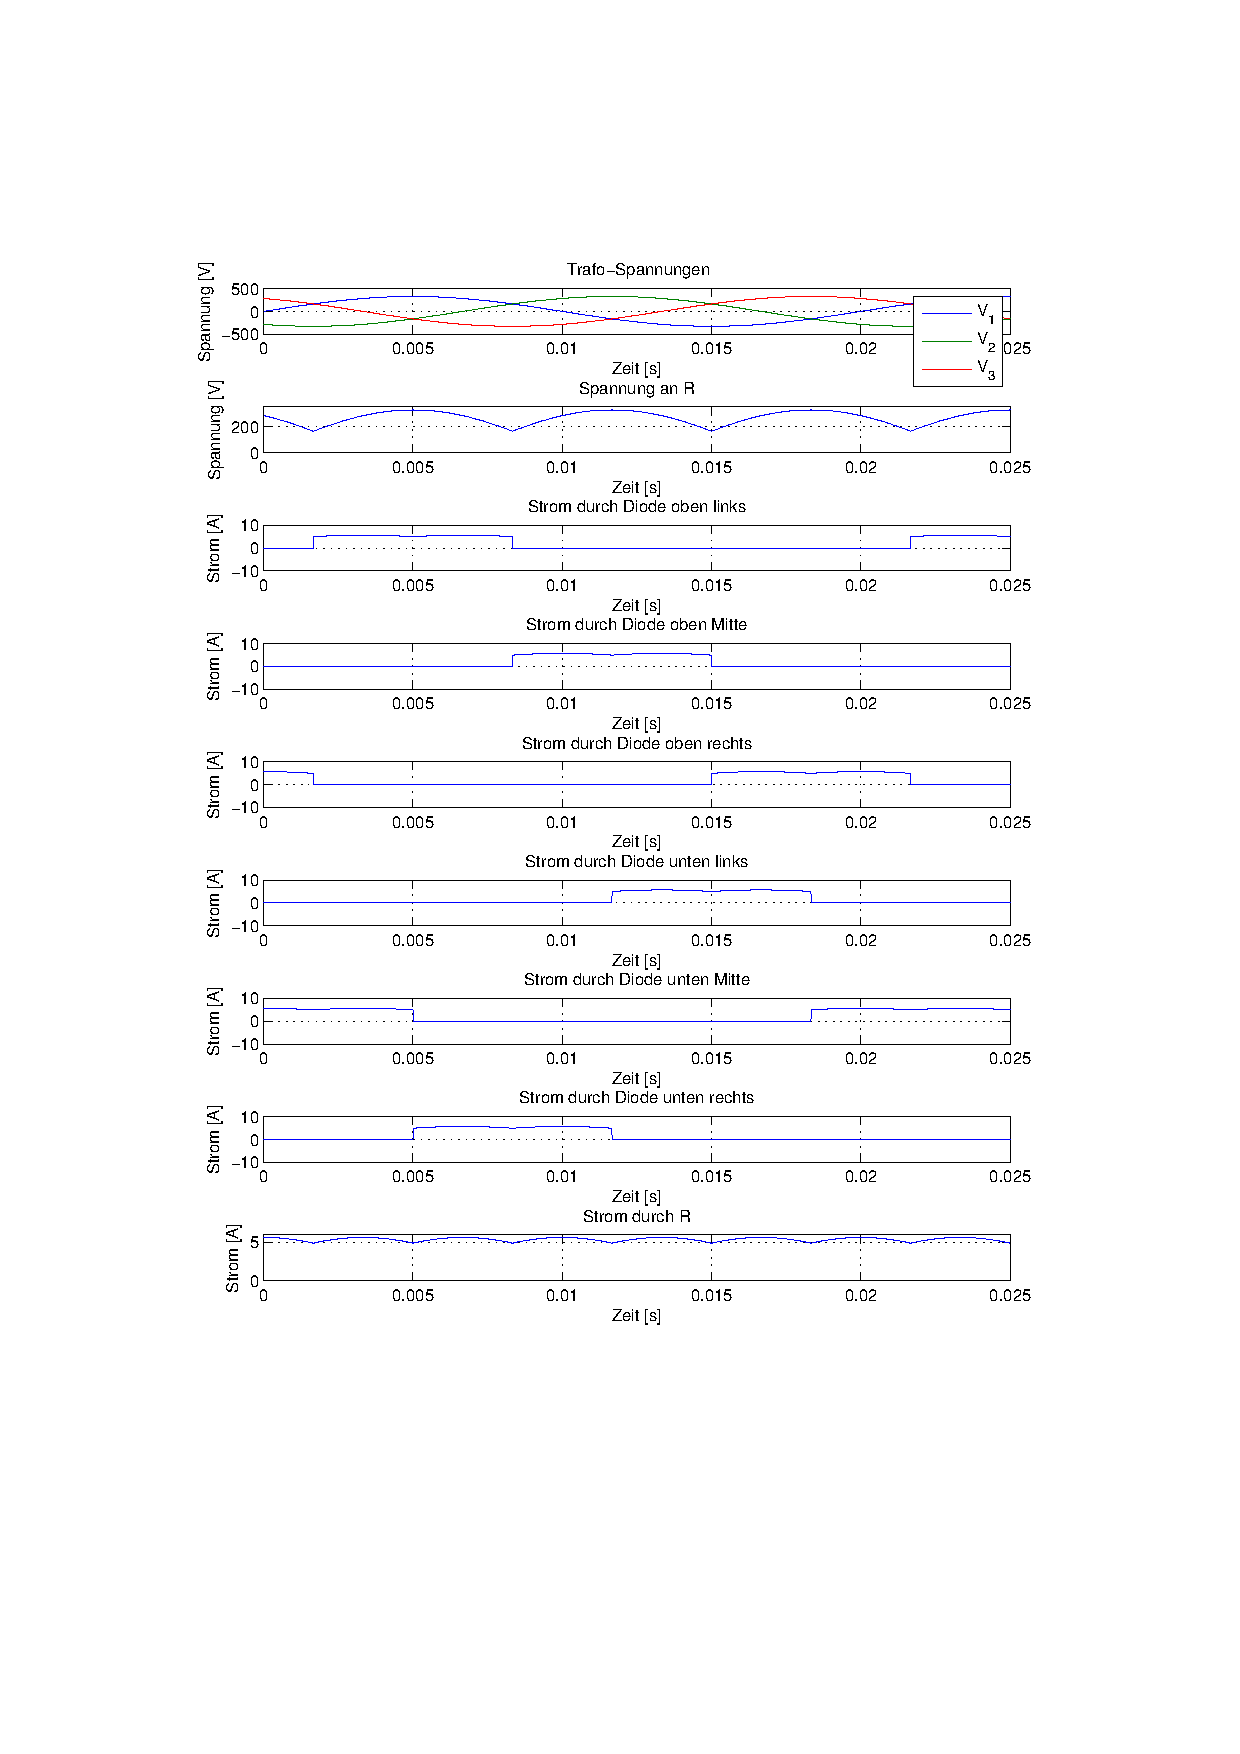
\includegraphics[width=6cm]{img/03-B6-Spannungsverlauf.pdf}
	
	$U_{\ir dia} = \frac{p}{2 \pi} \int \limits_{\frac{- \pi}{p} + a}^{\frac{\pi}{p} + a} \hat{U} \cos(\omega t) \diff \omega t = U_{\ir dia} \cos \alpha$
	
	!!!! Überprüfen
}

\section{DC-DC-Converters}
\sectionbox{
\subsection{Linearregler}
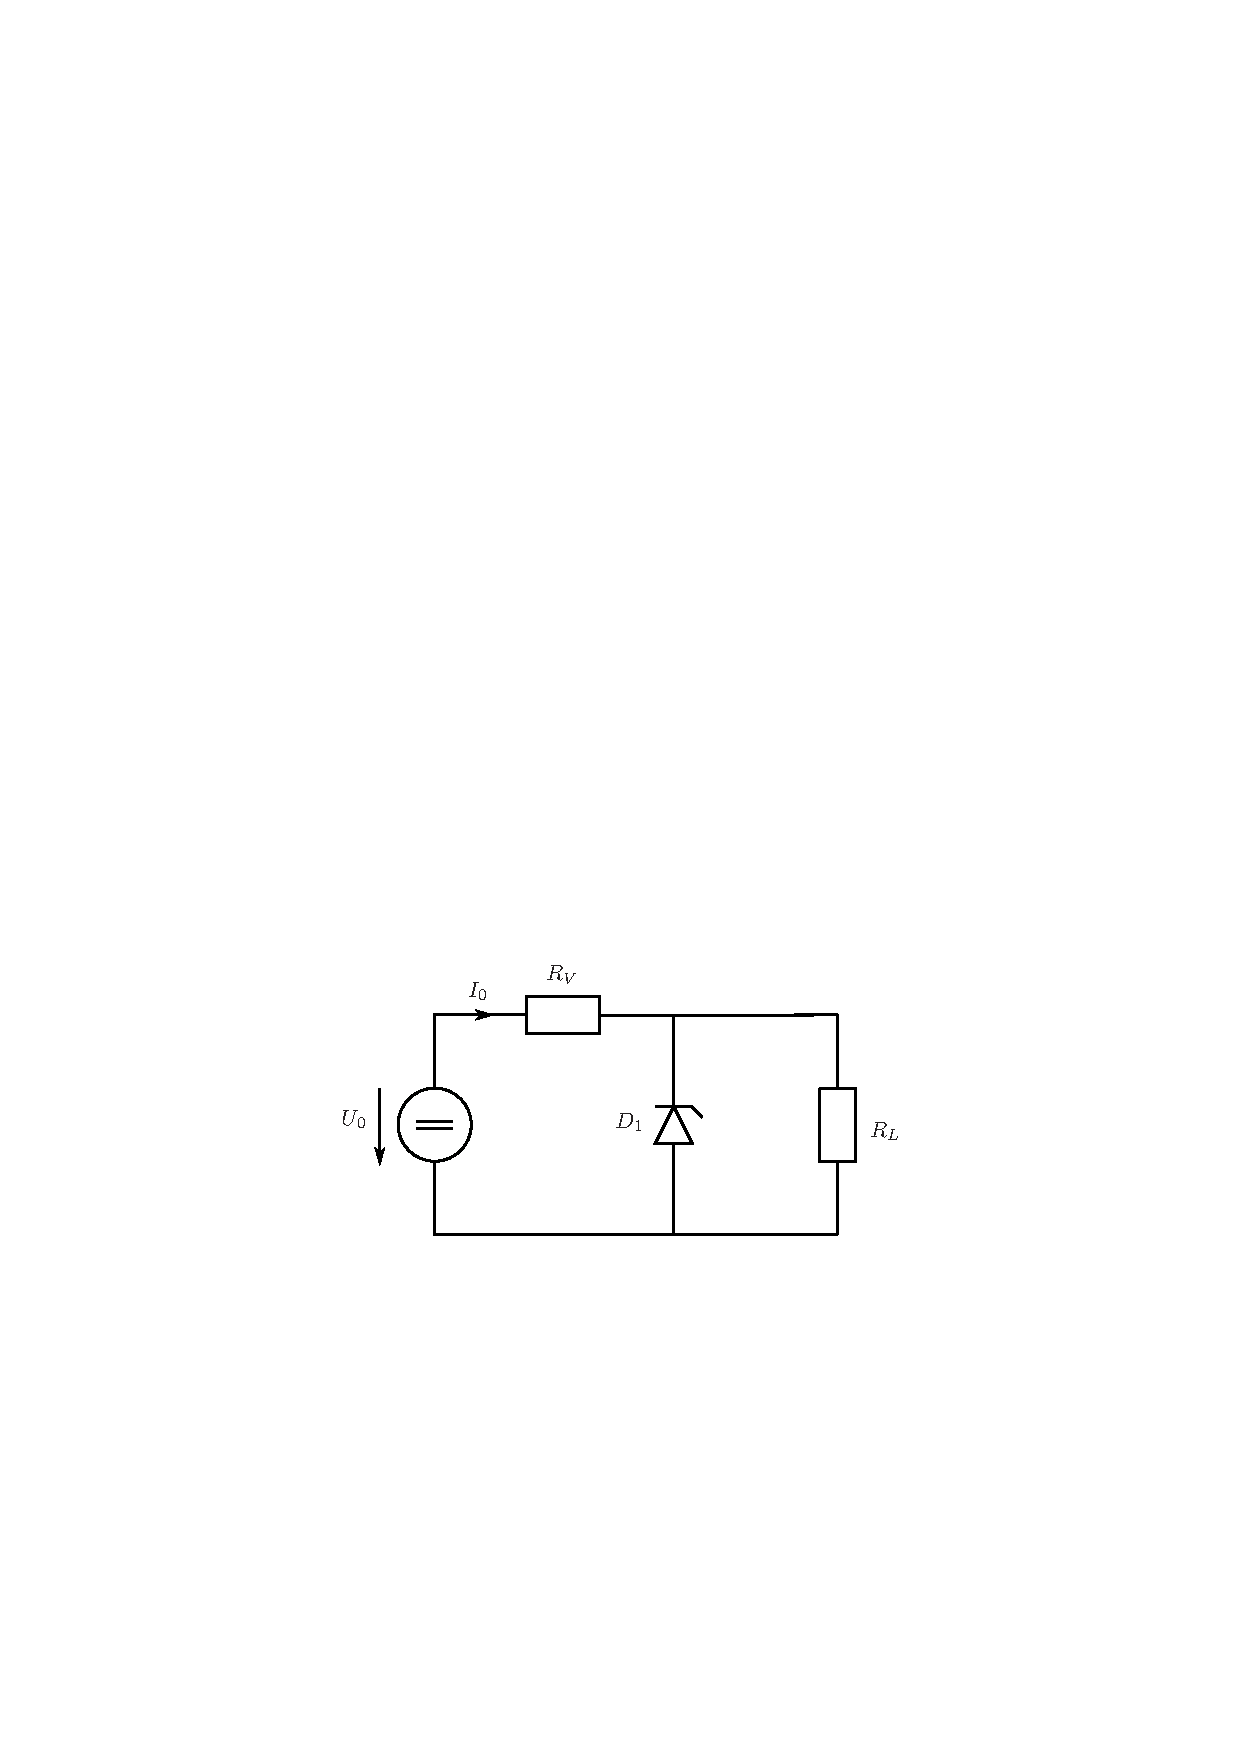
\includegraphics[width=5cm]{img/04-Linearregler.pdf}

\subsection{Tiefsetzsteller}
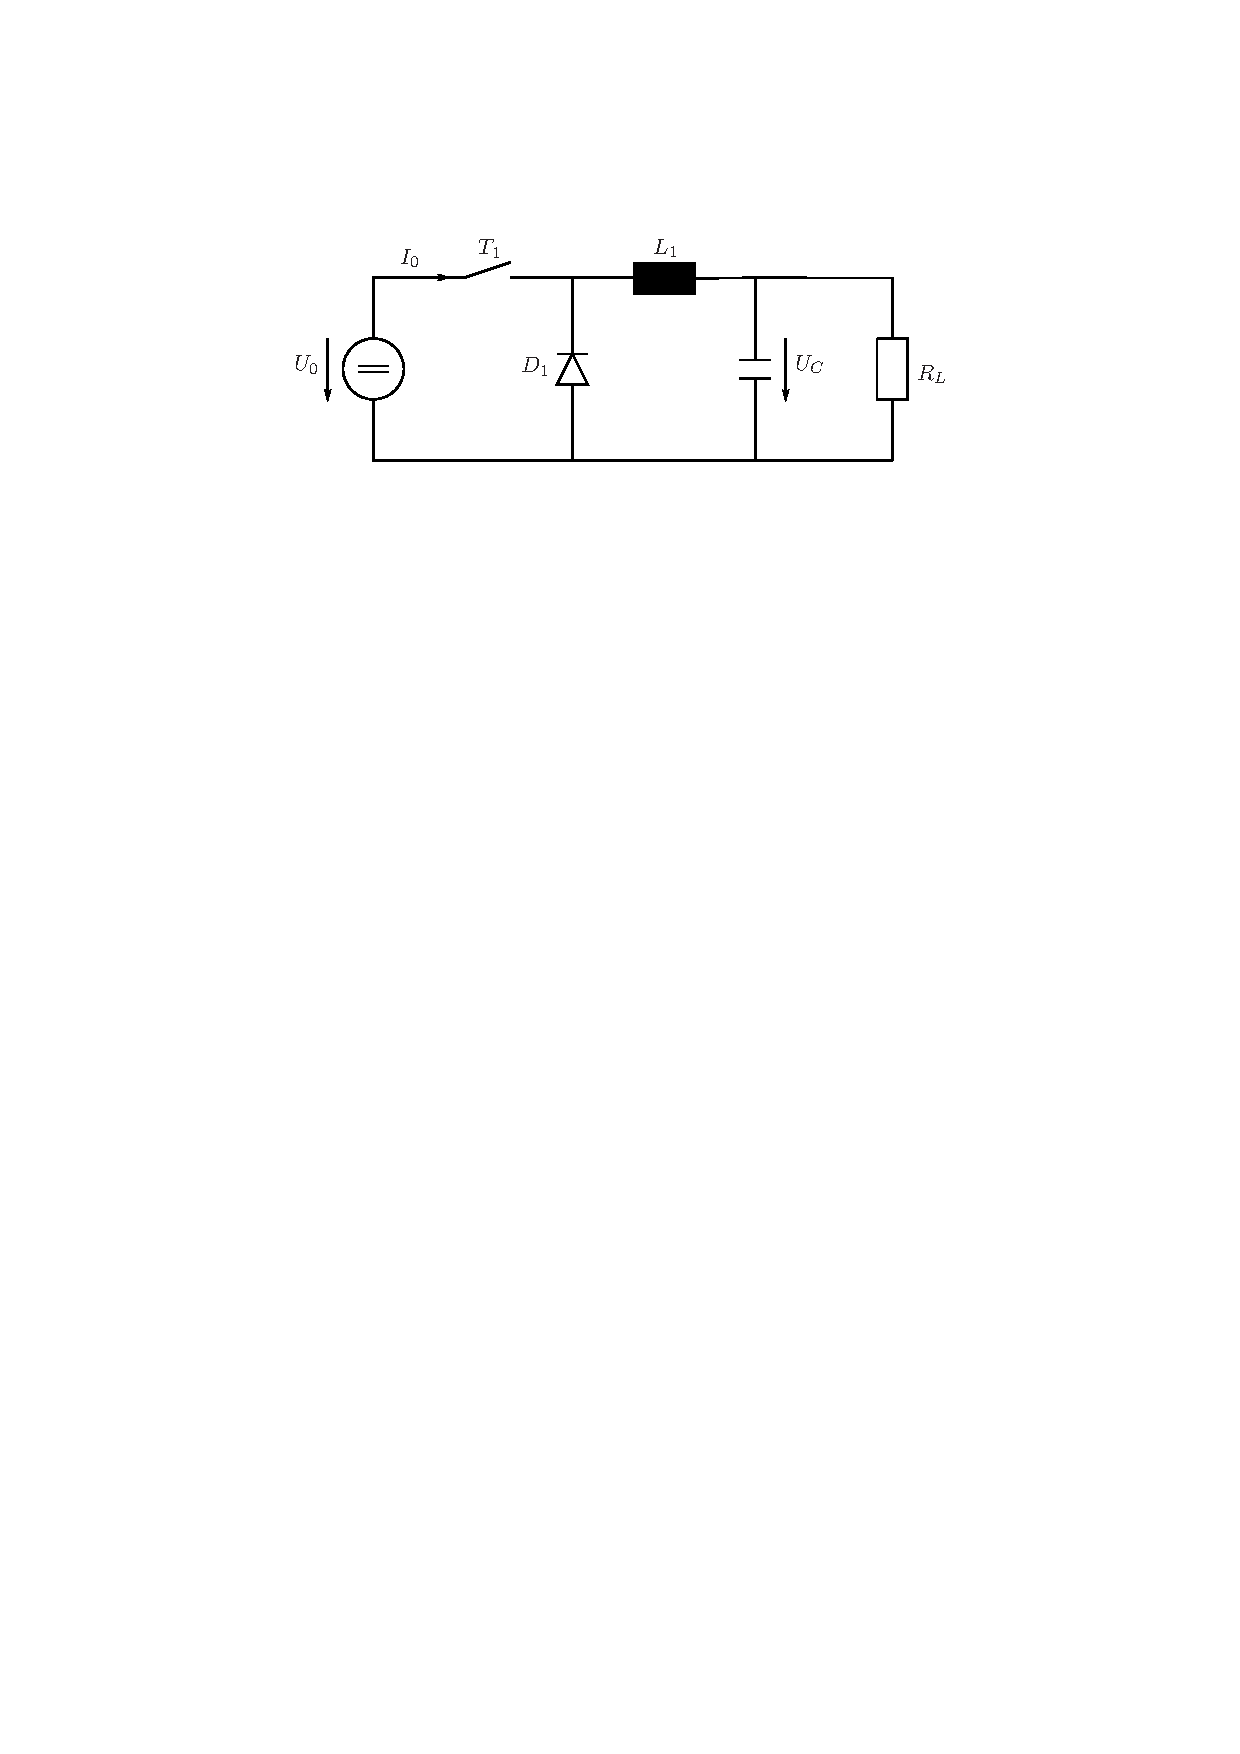
\includegraphics[width=5cm]{img/04-Tiefsetzstellers.pdf}

\subsection{Hochsetzsteller}
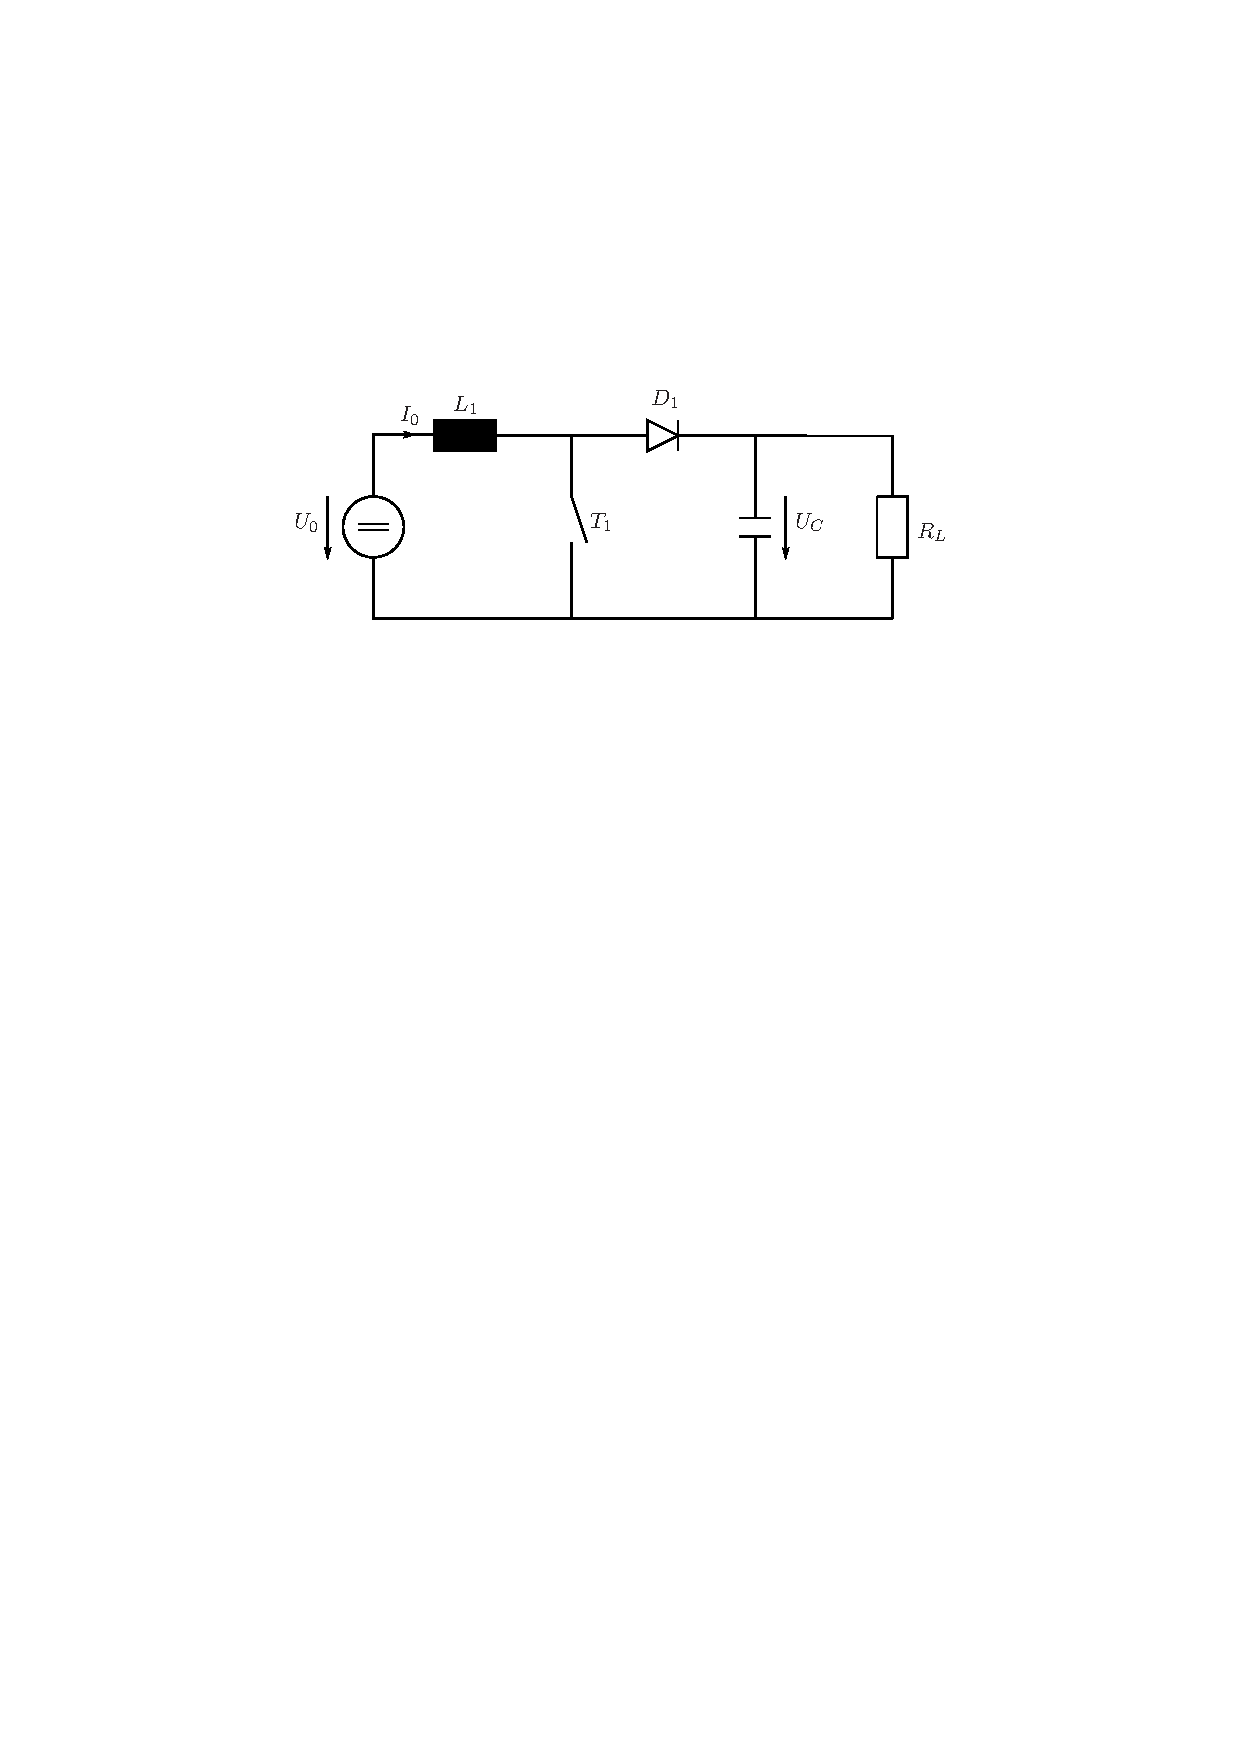
\includegraphics[width=5cm]{img/04-Hochsetzsteller.pdf}
}

\tiny{Bilder aus dem Übungsskript zum Fach Leistungselektronik: Grundlagen und Standartanwendungen
\copyright  Lehrstuhl für Elektrische Antriebssysteme und Leistungselektronik - TU München}



\section{Verluste}
\sectionbox{
	\subsection{Durchlassverluste} 

	zeitlicher Mittelwert: $I_{\ir AV} = \frac 1 T \int \limits_0^T i \diff t$

	Effektivwert: $I_{\ir RMS} = \sqrt{\frac 1 T \int \limits_0^T i^2 \diff t}$
}
\sectionbox{
	\subsection{Sperrverluste}

	für sinusförmige Sperrspannungen ($u_R (t) = \hat u_R \sin(\omega t)$)

	$P_R = \frac{1}{T} \int \limits_{0}^{T} p_R (t) \diff t  = \frac{1}{\pi} \hat u_R I_R$
}

\sectionbox{
	\subsection{Ein- und Ausschaltverluste}

	Einschaltverluste $W_{\ir on} = \int \limits_{t_0}^{t_0 + t_{\ir on}} p \diff t$

	Ausschaltverluste $W_{\ir off} = \int \limits_{t_0}^{t_0 + t_{\ir off}}$

	gesamte Schaltverluste $P_s = f(W_{\ir on} + W_{\ir off})$
}

\section{Thermisches Ersatzschaltbild}
\sectionbox{
\subsection{Wärmeleitung}
\symbolbox{
	\begin{tabular}{cc}
	 	$R_{\ir th}$ & Wärmewiderstand \\
	 	$\lambda$ & Wärmeleitfähigkeit \\
	 	$A$ & Querschnitt d. Körpers \\
	 	$d$ & Dicke des Körpers  
	\end{tabular}
}
Wärmeleitung: $R_{\ir th} = \frac{\theta_1 - \theta_2}{P}$

$R_{\ir th} = \frac{d}{\lambda A}$

}
\sectionbox{
\subsection{Wärmespeicherung}

\symbolbox{
	\begin{tabular}{cc}
	 	$C_{\ir th}	$& Wärmekapazität \\
	 	$V$ & Volumen \\
	 	$\gamma$ & spez. Masse \\
		$c$ & spez. Wärmekapazität
	\end{tabular}
}
$P = C_{\ir th} \frac{\diff \theta}{\diff t} = C_{\ir th} \theta$

$C_{\ir th} = V \gamma_C$
}

\sectionbox{
	\subsection{Transiente Wärmewiderstände}

}
% Ende der Spalten
\end{multicols*}

% Dokumentende
% ======================================================================
\end{document}

% ToDos:

